\chapter{Results}
In this chapter the results of multiple runs of the program will be discussed, both in 2D and 3D. First some runs in 2D will be discussed along with how the variables in the speed function affects the segmentation. Then some results from 3D runs will be illustrated, before the performance of different runs are compared. The Chan-Vese speed function implemented will not be discussed in any detail because the very simplified version implemented behaves much like a simple region grow function.
2D    
sirkelen og den andre greia -> full segmntering og..    

hjernebildet med chan-vese -> sammenlign med hjernebilde av vanlig speed funksjonen   

\section{2D}
First a simple binary image of size 512x512 of a circle shown in figure \ref{circle} was segmented. Values used: threshold ($T$) = 0.99, $\epsilon$ = 0.15 and $\alpha$ = 0.80. Since this image is binary the $T \pm \epsilon$ would not affect the end result of a full segmentation, as long as $T - \epsilon < 1 < T + \epsilon$. This also assumes that $T - \epsilon$ is not too close to 0, which would (also depending on $\alpha$) either stop the surface evolution midways or collaps it. The advantage of using higher values of $\epsilon$ within these limits is that higher values of $\epsilon$ makes the segmentation process faster by needing less iterations to achieve full segmentation. The reason is that the data term $D(I)$ (see \ref{dataFunction}) in the speed function is gradual, as mentioned when describing the speed function in chapter \ref{levelSetChap}.
\begin{figure}[h!]
\centering
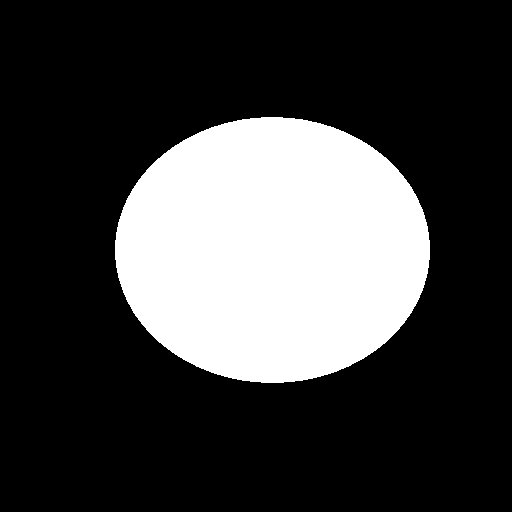
\includegraphics[width=0.65\textwidth]{results/2D/circle}
\caption{Input: simple binary image}
\label{circle}
\end{figure} 

Figure \ref{circleZero0} illustrates the zero level set (and a zoomed in version in the top-right corner) right after its initialization where a circular zero level set was created with center in coordinate (235,235) and with radius = 10. 
\begin{figure}[h!]
\centering
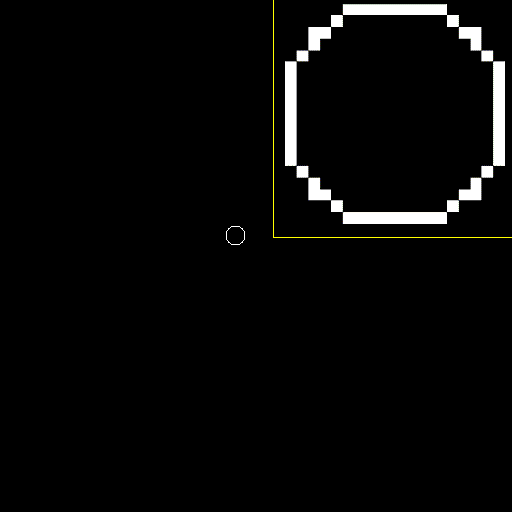
\includegraphics[width=0.65\textwidth]{results/2D/circleZero0}
\caption{Zero level set right after initialization}
\label{circleZero0}
\end{figure} 

Figures \ref{circleZeroMany} a, b and c represents the zero level set after 700, 1200 and 1600 iterations respectively. Figure \ref{circleZeroMany}d illustrates the full segmentation result which required 2200 iterations.

\begin{figure}[h!]
\centering
\begin{minipage}{.49\textwidth}
\begin{tabular}{c}

\includegraphics[width=.9\textwidth]{results/2D/circleZero700} \\
(a)
\end{tabular}
\end{minipage}
\begin{minipage}{.49\textwidth}
\begin{tabular}{c}
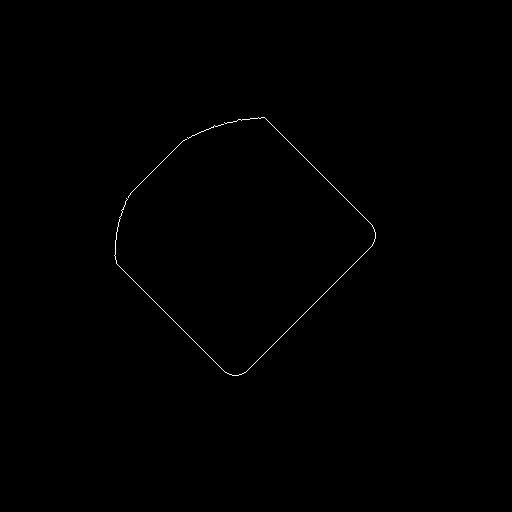
\includegraphics[width=.9\textwidth]{results/2D/circleZero1200} \\
(b)
\end{tabular}
\end{minipage}
\\
\begin{minipage}{.49\textwidth}
\begin{tabular}{c}
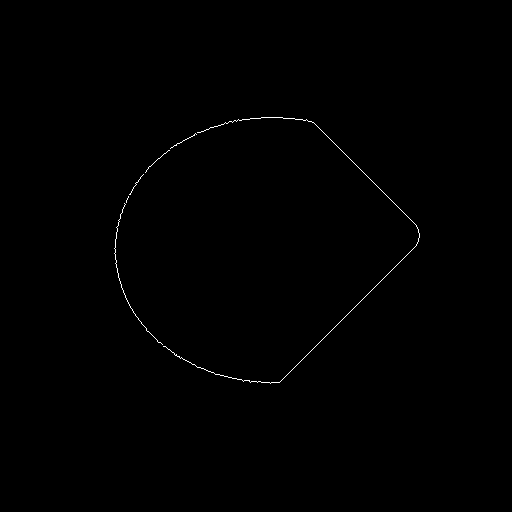
\includegraphics[width=.9\textwidth]{results/2D/circleZero1600} \\
(c)
\end{tabular}
\end{minipage}
\begin{minipage}{.49\textwidth}
\begin{tabular}{c}
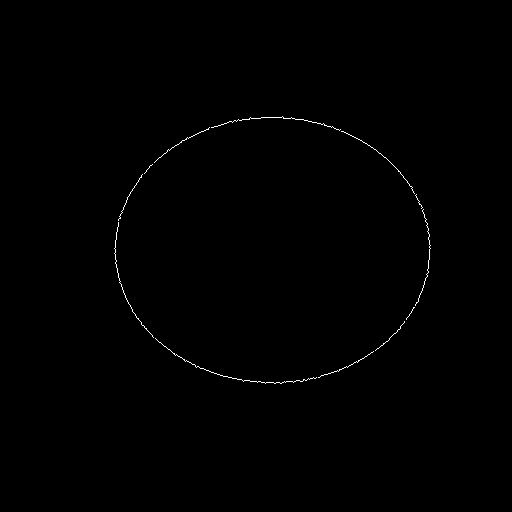
\includegraphics[width=.9\textwidth]{results/2D/circleZero2200_full} \\
(d)
\end{tabular}
\end{minipage}
\\
\begin{minipage}{.49\textwidth}
\begin{tabular}{c}

\includegraphics[width=.9\textwidth]{results/2D/circleEps005} \\
(e)
\end{tabular}
\end{minipage}
\caption{Zero level set after: (a): 600, (b): 1200, (c): 1600 and (d): 2200 iterations (e): with $\epsilon=0.05$.}
\label{circleZeroMany}
\end{figure}
Comparing the input image in figure \ref{circle} and the segmentation result in figure \ref{circleZeroMany}d it can be seen that the program succesfully segmented the image.
Another segmentation, with all variables equal to the previous segmentation except for $\epsilon$, was run to measure the difference in iterations needed to get a full segmentation. By assigning the $\epsilon$ a value 0.05 the result was the exact same after full segmentation, but the numbers of iterations increased from 2200 to about 8600 iteratuins, an increase of nearly four times. By omparing figure \ref{circleZeroMany}d with figure \ref{circleZeroMany}e which is the result after 2200 iterations with $\epsilon$ = 0.05 it can be seen how much slower the interface evolves.
To test if the program works as it should when parts of the seed point is outside the object to be segmented, the seed point was as shown in red in figure \ref{circleSeedPartlyOutside}a where it is superimposed on the input image. How the interface looked like after 300, 800 and 1300 iterations is depicted in figure \ref{circleSeedPartlyOutside}b, c and d respectively. The final segmentation result was as expected a correct segmentation of the object as in figure \ref{circleZeroMany}d. 
\begin{figure}[h!]
\centering
\begin{minipage}{.49\textwidth}
\begin{tabular}{c}
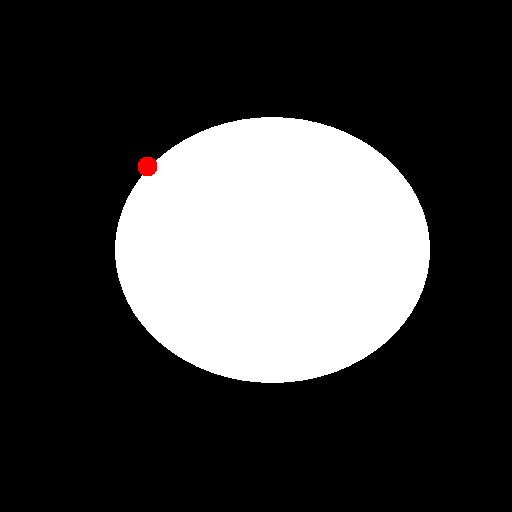
\includegraphics[width=.9\textwidth]{results/2D/circleSeedPartlyOutside} \\
(a)
\end{tabular}
\end{minipage}
\begin{minipage}{.49\textwidth}
\begin{tabular}{c}
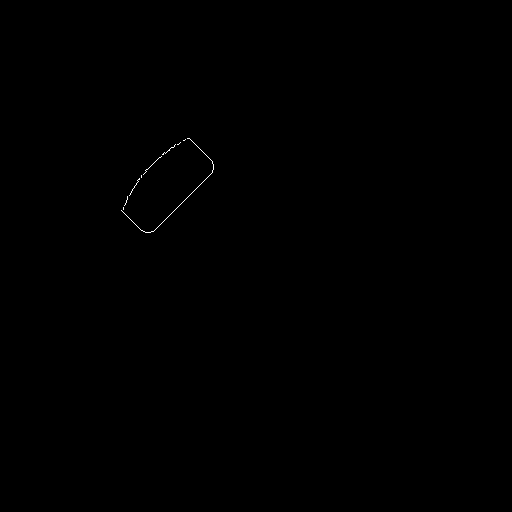
\includegraphics[width=.9\textwidth]{results/2D/circleSeedPartlyOutside300} \\
(b)
\end{tabular}
\end{minipage}
\\
\begin{minipage}{.49\textwidth}
\begin{tabular}{c}
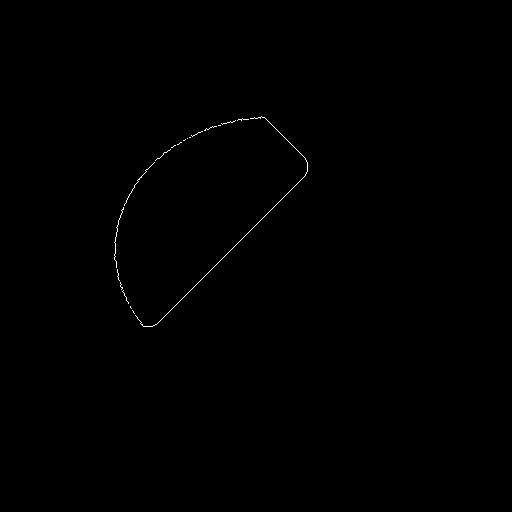
\includegraphics[width=.9\textwidth]{results/2D/circleSeedPartlyOutside800} \\
(c)
\end{tabular}
\end{minipage}
\begin{minipage}{.49\textwidth}
\begin{tabular}{c}
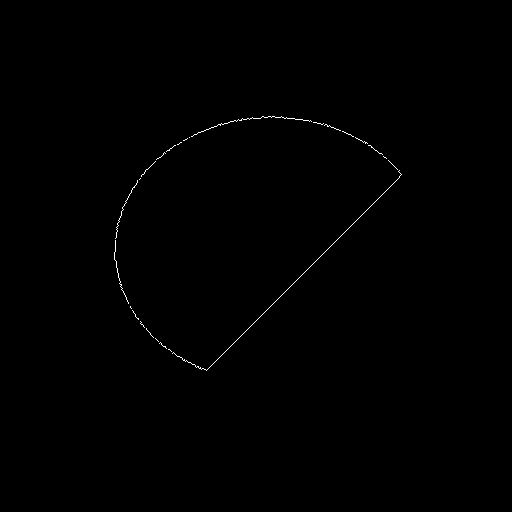
\includegraphics[width=.9\textwidth]{results/2D/circleSeedPartlyOutside1300} \\
(d)
\end{tabular}
\end{minipage}
\caption{(a): Seed point partly outside the object, superimposed on the input image. Interface after (b): 300, (c): 800 and (d): 1300 iterations.}
\label{circleZeroMany}
\end{figure}

To further test the robustness of the program and to illustrate the effect $\alpha$ has on the smoothness of the interface the 512x512 binary image in figure \ref{randOrgWSeed}a, with the seed point superimposed in red, was segmented. Notice the one-pixel wide "cut" at the top that seperates the main object in the image from the smaller one. Also notice the one-pixel wide line that holds together the main object with the ractangle at the button. Two full segmentations were run, both with $T$ = 0.99 and $\epsilon$ = 0.15, but figure \ref{randOrgWSeed}b is the result with $\alpha$ = 0.80 and \ref{randOrgWSeed}c with $\alpha$ = 0.90.
\begin{figure}[h!]
\centering
\begin{minipage}{.49\textwidth}
\begin{tabular}{c}
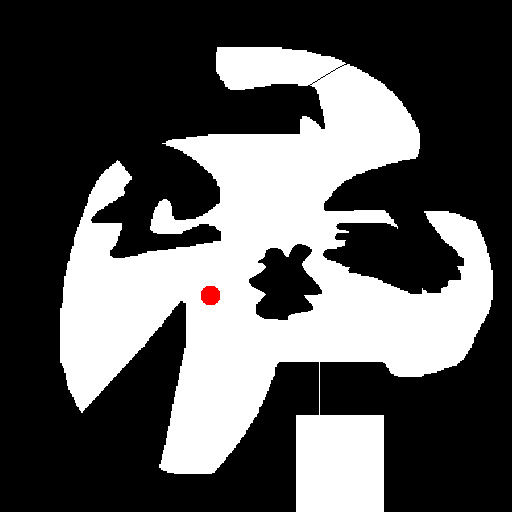
\includegraphics[width=.9\textwidth]{results/2D/randOrgWSeed} \\
(a)
\end{tabular}
\end{minipage}
\\
\begin{minipage}{.49\textwidth}
\begin{tabular}{c}
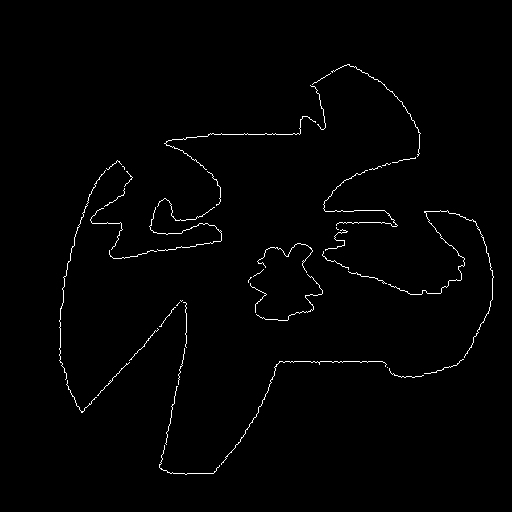
\includegraphics[width=.9\textwidth]{results/2D/randOrgWSeeda080} \\
(b)
\end{tabular}
\end{minipage}
\begin{minipage}{.49\textwidth}
\begin{tabular}{c}
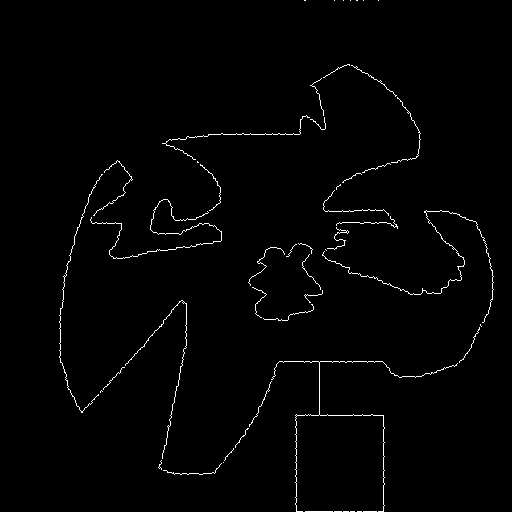
\includegraphics[width=.9\textwidth]{results/2D/randOrgWSeeda090} \\
(c)
\end{tabular}
\end{minipage}
\caption{(a): Input image with seed point superimposed. Segmentation result with (b): $\alpha$ = 0.80, (c): $\alpha$ = 0.90.}
\label{randOrgWSeed}
\end{figure}
As explained in chapter \ref{levelSetChap}, $\alpha$ restricts how much the interface can bend and prevents the model from leaking into unwanted areas, which can be seen by the fact that \ref{randOrgWSeed}c with a higer value of $\alpha$ have been able to include the rectangle at the button by evolving through the thin line, while \ref{randOrgWSeed}b with only a value of 0.10 $\alpha$ less did not manage it. Higher values gives more importance to \(D(I)\) and lower values makes \(\nabla \frac{\nabla \phi}{|\nabla \phi|}\) affect the level set more. The more importance \(\nabla \frac{\nabla \phi}{|\nabla \phi|}\) gets, the less likely is the model to leak into unwanted areas. But giving \(\nabla \frac{\nabla \phi}{|\nabla \phi|}\) too much importance makes the model so smooth that it does not reach all areas of the object being segmented, which is illustrated in \ref{starZero}b with $\alpha$ = 0.4 and \ref{starZero}a was used as input image. Figures \ref{starZero}a and b are small of size (100x100) to be able to more clearly illustrate the difference in input image and segmented image when the smoothness is highly valued.
\begin{figure}[h!]
\centering
\begin{minipage}{.39\textwidth}
\begin{tabular}{c}

\includegraphics[width=.9\textwidth]{results/2D/starZero} \\
(a)
\end{tabular}
\end{minipage}
\begin{minipage}{.39\textwidth}
\begin{tabular}{c}

\includegraphics[width=.9\textwidth]{results/2D/starZeroFullSeg} \\
(b)
\end{tabular}
\end{minipage}
\caption{Interface smoothness highly valued. (a): Input image, (b): segmentation result.}
\label{starZero}
\end{figure}

\section{3D}
First volume to be segmented  was a volume of an aneurism in a "semi segmented brain volume". 
\begin{figure}[h!]
\centering
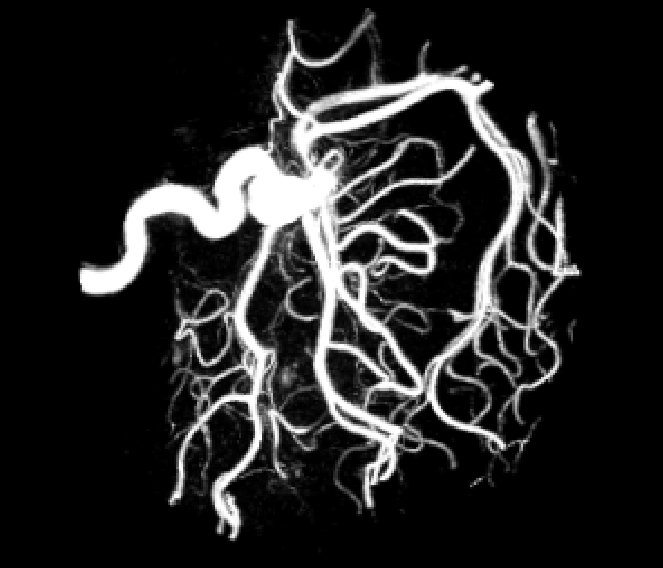
\includegraphics[width=.9\textwidth]{results/3D/3D-aneurism-unsegmented/aneurism_original_mip}
\label{aneurism_original}
\caption{Maximum intensity projection of the volume to be segmented}
\end{figure}
The goal was to segment the aneurism itself as well as adjacent arteries without expanding into insignificant parts of the volume. In figure \ref{aneurism_original} we can see the maximum intensity projection of the unsegmented volume. The part we want to segment is an aneurism on the arterie located inside the brain (not shown in the picture) and adjacent arteries. Not only is the segmentation used to extract important features of the aneurism in order to help surgeons make decisions as to how to operate on it. By also adding sections of the connecting veins, registration can be performed by trying to find a one to one correspondence between the model and samples of the patient on the table, which is then used as a reference frame during computer aided surgery. 


Figure \ref{aneurism_500_iterations} shows how segmentation of the image looks like after 500 iterations. The values of T, $\epsilon$, and $\alpha$ used is T = 1.0, $\epsilon$ = 0.3 and $\alpha$ = 0.75. 
\begin{figure}[h!]
\centering
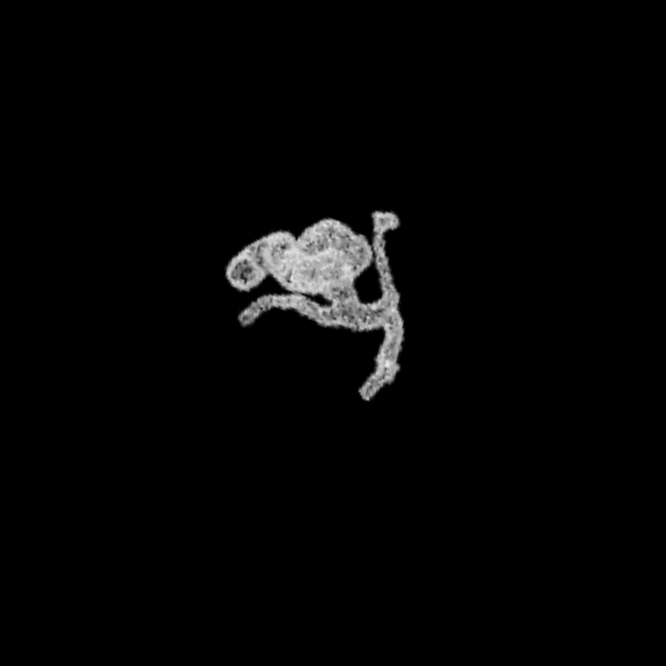
\includegraphics[width=.9\textwidth]{results/3D/aneurism_500_iterations}
\label{aneurism_500_iterations}
\caption{Aneurism segmentation after 500 iterations.}
\end{figure}
The aneurism volume has dimensions 256x256x256 and the maximal speed the interface can have using sparse field is 1. In theory this would mean that we only need about half the number of iterations as the biggest image dimension (assuming the seed point is located near the center of the volume) in order to achieve convergence. In practice the speed is reduced by both the curcature and the . It turns out that to achieve a satisfying result given the input parameters stated above, about 3000 iterations is needed. Figure 3 shows the segmentated volume after 500, 1000 and 1500 iterations of the volume. The white part of the structure is the volume segmented after 500 iterations. The light blue colored part shows the segmentation after 1000 iterations and the darker blue shows the segmented volume after 1500 iterations. The figure shows how stable the algorithm is throughout the run. The area along the walls of the arteries covered after 500 iterations is not retracting at a later point, nor is it expanding further. This is shown by observing how well the 500 iterations volume and the 1500 iterations volume overlap.

Next we have the segmented volume after 2000 and 3000 iterations in figure 4, which has colors red and green respectively. The overlapping areas are indicated in yellow. As we can see the last 1000 iterations is not a huge improvement, but the volume is definitely not at equilibrium after 2000 iterations. 
\\
We also tested the data on a CT volume of an abdomen to extract the volume of the liver. This is somewhat tricky because the liver has greyscale values very similar to the organs surrounding it and so it is difficult to prevent the interface from leaking into the surroundings. And altho the curvature term will prevent pixel sized leaks and small holes, it will not prevent a broad part of the interface to move out of the liver volume unless the curvatures is weighted heavily. In addition, the internal structures of the liver migh vary even more than the liver and its surroundings. So the parameters has to be chosen wisely to get a good segmentation. Figure CT z axis shows a slice in the z axis of the volume. The liver is the big semi-uniform area that stretches from the left and over the middle of the stomach. As we can see the difference in the pixel values between the liver area and its surroundings are small. The dimensions of the image are 320x220x72. Next we see the segmented volume (figure ct with poor threshold) using values (insert values for liver CT) and (insert iterations) iterations. The threshold in this image (reference figure ct with poor threshold) is too high and so the 

\section{Performance}
TODO 
HELT til slutt i kapittelet: en tabell med antall iterasjoner og tid brukt på alle segmenteringene, både 2D og 3D (eventuelt også CUDA). The results in this table were all aquired by using a single seed point set at an optimal location close to the center of the object being segmented, with a radius of 10. The variable values used were found to be the fastest ones, given a specific object, while resulting in a correct and complete segmentation. The time was taken for only the segmentation process, thus not including the time used to read input, initialize and write result back to file.